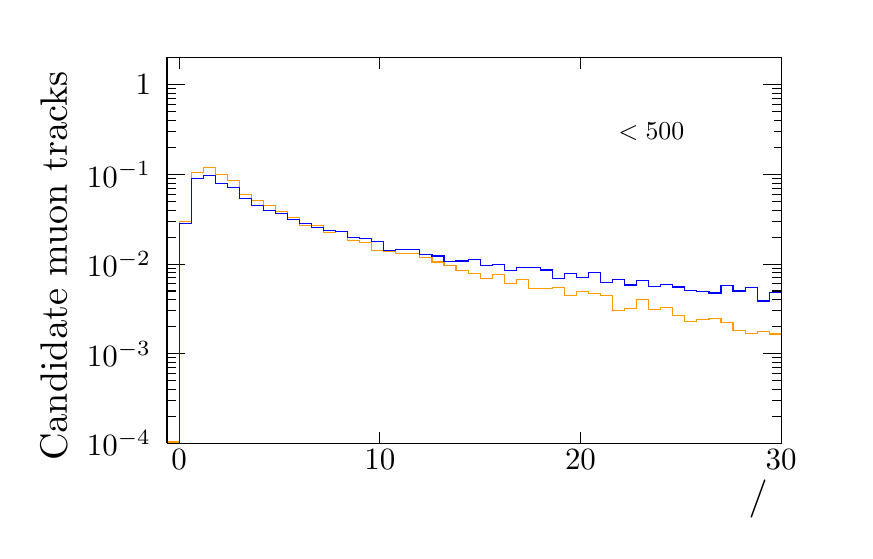
\begin{tikzpicture}
\pgfdeclareplotmark{cross} {
\pgfpathmoveto{\pgfpoint{-0.3\pgfplotmarksize}{\pgfplotmarksize}}
\pgfpathlineto{\pgfpoint{+0.3\pgfplotmarksize}{\pgfplotmarksize}}
\pgfpathlineto{\pgfpoint{+0.3\pgfplotmarksize}{0.3\pgfplotmarksize}}
\pgfpathlineto{\pgfpoint{+1\pgfplotmarksize}{0.3\pgfplotmarksize}}
\pgfpathlineto{\pgfpoint{+1\pgfplotmarksize}{-0.3\pgfplotmarksize}}
\pgfpathlineto{\pgfpoint{+0.3\pgfplotmarksize}{-0.3\pgfplotmarksize}}
\pgfpathlineto{\pgfpoint{+0.3\pgfplotmarksize}{-1.\pgfplotmarksize}}
\pgfpathlineto{\pgfpoint{-0.3\pgfplotmarksize}{-1.\pgfplotmarksize}}
\pgfpathlineto{\pgfpoint{-0.3\pgfplotmarksize}{-0.3\pgfplotmarksize}}
\pgfpathlineto{\pgfpoint{-1.\pgfplotmarksize}{-0.3\pgfplotmarksize}}
\pgfpathlineto{\pgfpoint{-1.\pgfplotmarksize}{0.3\pgfplotmarksize}}
\pgfpathlineto{\pgfpoint{-0.3\pgfplotmarksize}{0.3\pgfplotmarksize}}
\pgfpathclose
\pgfusepathqstroke
}
\pgfdeclareplotmark{cross*} {
\pgfpathmoveto{\pgfpoint{-0.3\pgfplotmarksize}{\pgfplotmarksize}}
\pgfpathlineto{\pgfpoint{+0.3\pgfplotmarksize}{\pgfplotmarksize}}
\pgfpathlineto{\pgfpoint{+0.3\pgfplotmarksize}{0.3\pgfplotmarksize}}
\pgfpathlineto{\pgfpoint{+1\pgfplotmarksize}{0.3\pgfplotmarksize}}
\pgfpathlineto{\pgfpoint{+1\pgfplotmarksize}{-0.3\pgfplotmarksize}}
\pgfpathlineto{\pgfpoint{+0.3\pgfplotmarksize}{-0.3\pgfplotmarksize}}
\pgfpathlineto{\pgfpoint{+0.3\pgfplotmarksize}{-1.\pgfplotmarksize}}
\pgfpathlineto{\pgfpoint{-0.3\pgfplotmarksize}{-1.\pgfplotmarksize}}
\pgfpathlineto{\pgfpoint{-0.3\pgfplotmarksize}{-0.3\pgfplotmarksize}}
\pgfpathlineto{\pgfpoint{-1.\pgfplotmarksize}{-0.3\pgfplotmarksize}}
\pgfpathlineto{\pgfpoint{-1.\pgfplotmarksize}{0.3\pgfplotmarksize}}
\pgfpathlineto{\pgfpoint{-0.3\pgfplotmarksize}{0.3\pgfplotmarksize}}
\pgfpathclose
\pgfusepathqfillstroke
}
\pgfdeclareplotmark{newstar} {
\pgfpathmoveto{\pgfqpoint{0pt}{\pgfplotmarksize}}
\pgfpathlineto{\pgfqpointpolar{44}{0.5\pgfplotmarksize}}
\pgfpathlineto{\pgfqpointpolar{18}{\pgfplotmarksize}}
\pgfpathlineto{\pgfqpointpolar{-20}{0.5\pgfplotmarksize}}
\pgfpathlineto{\pgfqpointpolar{-54}{\pgfplotmarksize}}
\pgfpathlineto{\pgfqpointpolar{-90}{0.5\pgfplotmarksize}}
\pgfpathlineto{\pgfqpointpolar{234}{\pgfplotmarksize}}
\pgfpathlineto{\pgfqpointpolar{198}{0.5\pgfplotmarksize}}
\pgfpathlineto{\pgfqpointpolar{162}{\pgfplotmarksize}}
\pgfpathlineto{\pgfqpointpolar{134}{0.5\pgfplotmarksize}}
\pgfpathclose
\pgfusepathqstroke
}
\pgfdeclareplotmark{newstar*} {
\pgfpathmoveto{\pgfqpoint{0pt}{\pgfplotmarksize}}
\pgfpathlineto{\pgfqpointpolar{44}{0.5\pgfplotmarksize}}
\pgfpathlineto{\pgfqpointpolar{18}{\pgfplotmarksize}}
\pgfpathlineto{\pgfqpointpolar{-20}{0.5\pgfplotmarksize}}
\pgfpathlineto{\pgfqpointpolar{-54}{\pgfplotmarksize}}
\pgfpathlineto{\pgfqpointpolar{-90}{0.5\pgfplotmarksize}}
\pgfpathlineto{\pgfqpointpolar{234}{\pgfplotmarksize}}
\pgfpathlineto{\pgfqpointpolar{198}{0.5\pgfplotmarksize}}
\pgfpathlineto{\pgfqpointpolar{162}{\pgfplotmarksize}}
\pgfpathlineto{\pgfqpointpolar{134}{0.5\pgfplotmarksize}}
\pgfpathclose
\pgfusepathqfillstroke
}
\definecolor{c}{rgb}{1,1,1};
\draw [color=c, fill=c] (0,0) rectangle (10,6.27517);
\draw [color=c, fill=c] (1.4,1.00403) rectangle (9.2,5.89866);
\definecolor{c}{rgb}{0,0,0};
\draw [c] (1.4,1.00403) -- (1.4,5.89866) -- (9.2,5.89866) -- (9.2,1.00403) -- (1.4,1.00403);
\definecolor{c}{rgb}{1,1,1};
\draw [color=c, fill=c] (1.4,1.00403) rectangle (9.2,5.89866);
\definecolor{c}{rgb}{0,0,0};
\draw [c] (1.4,1.00403) -- (1.4,5.89866) -- (9.2,5.89866) -- (9.2,1.00403) -- (1.4,1.00403);
\definecolor{c}{rgb}{1,0.6,0};
\draw [c,line width=0.4] (1.41678,1.02081) -- (1.41678,1.02081) -- (1.55294,1.02081) -- (1.55294,3.82277) -- (1.70588,3.82277) -- (1.70588,4.43859) -- (1.85882,4.43859) -- (1.85882,4.50284) -- (2.01176,4.50284) -- (2.01176,4.41416) --
 (2.16471,4.41416) -- (2.16471,4.3398) -- (2.31765,4.3398) -- (2.31765,4.16077) -- (2.47059,4.16077) -- (2.47059,4.08455) -- (2.62353,4.08455) -- (2.62353,4.0208) -- (2.77647,4.0208) -- (2.77647,3.95189) -- (2.92941,3.95189) -- (2.92941,3.8718) --
 (3.08235,3.8718) -- (3.08235,3.77058) -- (3.23529,3.77058) -- (3.23529,3.77338) -- (3.38824,3.77338) -- (3.38824,3.68092) -- (3.54118,3.68092) -- (3.54118,3.68894) -- (3.69412,3.68894) -- (3.69412,3.57799) -- (3.84706,3.57799) -- (3.84706,3.55246)
 -- (4,3.55246) -- (4,3.45638) -- (4.15294,3.45638) -- (4.15294,3.44021) -- (4.30588,3.44021) -- (4.30588,3.41202) -- (4.45882,3.41202) -- (4.45882,3.41086) -- (4.61176,3.41086) -- (4.61176,3.36201) -- (4.76471,3.36201) -- (4.76471,3.30636) --
 (4.91765,3.30636) -- (4.91765,3.26126) -- (5.07059,3.26126) -- (5.07059,3.19751) -- (5.22353,3.19751) -- (5.22353,3.16418) -- (5.37647,3.16418) -- (5.37647,3.09212) -- (5.52941,3.09212) -- (5.52941,3.14861) -- (5.68235,3.14861) -- (5.68235,3.02834)
 -- (5.83529,3.02834) -- (5.83529,3.08318) -- (5.98824,3.08318) -- (5.98824,2.97233) -- (6.14118,2.97233) -- (6.14118,2.96665) -- (6.29412,2.96665) -- (6.29412,2.98073) -- (6.44706,2.98073) -- (6.44706,2.88616) -- (6.6,2.88616) -- (6.6,2.93722) --
 (6.75294,2.93722) -- (6.75294,2.90269) -- (6.90588,2.90269) -- (6.90588,2.88278) -- (7.05882,2.88278) -- (7.05882,2.69575) -- (7.21176,2.69575) -- (7.21176,2.71986) -- (7.36471,2.71986) -- (7.36471,2.8292) -- (7.51765,2.8292) -- (7.51765,2.70067) --
 (7.67059,2.70067) -- (7.67059,2.72919) -- (7.82353,2.72919) -- (7.82353,2.62692) -- (7.97647,2.62692) -- (7.97647,2.55357) -- (8.12941,2.55357) -- (8.12941,2.57925) -- (8.28235,2.57925) -- (8.28235,2.58546) -- (8.43529,2.58546) -- (8.43529,2.54021)
 -- (8.58823,2.54021) -- (8.58823,2.43497) -- (8.74118,2.43497) -- (8.74118,2.40028) -- (8.89412,2.40028) -- (8.89412,2.42653) -- (9.04706,2.42653) -- (9.04706,2.39121) -- (9.2,2.39121) -- (9.2,1.02081);
\definecolor{c}{rgb}{0,0,0};
\draw [c,line width=0.4] (1.4,1.00403) -- (9.2,1.00403);
\draw [anchor= east] (9.2,0.301208) node[scale=1.37879, rotate=0]{$\chisq/\nDoF$};
\draw [c,line width=0.4] (1.55294,1.15087) -- (1.55294,1.00403);
\draw [c,line width=0.4] (4.10196,1.15087) -- (4.10196,1.00403);
\draw [c,line width=0.4] (6.65098,1.15087) -- (6.65098,1.00403);
\draw [c,line width=0.4] (9.2,1.15087) -- (9.2,1.00403);
\draw [c,line width=0.4] (1.55294,1.15087) -- (1.55294,1.00403);
\draw [anchor=base] (1.55294,0.665168) node[scale=1.11794, rotate=0]{0};
\draw [anchor=base] (4.10196,0.665168) node[scale=1.11794, rotate=0]{10};
\draw [anchor=base] (6.65098,0.665168) node[scale=1.11794, rotate=0]{20};
\draw [anchor=base] (9.2,0.665168) node[scale=1.11794, rotate=0]{30};
\draw [c,line width=0.4] (1.4,5.89866) -- (9.2,5.89866);
\draw [c,line width=0.4] (1.55294,5.75182) -- (1.55294,5.89866);
\draw [c,line width=0.4] (4.10196,5.75182) -- (4.10196,5.89866);
\draw [c,line width=0.4] (6.65098,5.75182) -- (6.65098,5.89866);
\draw [c,line width=0.4] (9.2,5.75182) -- (9.2,5.89866);
\draw [c,line width=0.4] (1.55294,5.75182) -- (1.55294,5.89866);
\draw [c,line width=0.4] (1.4,1.00403) -- (1.4,5.89866);
\draw [anchor= east] (-0.04,5.89866) node[scale=1.37879, rotate=90]{Candidate muon tracks};
\draw [c,line width=0.4] (1.634,1.00403) -- (1.4,1.00403);
\draw [anchor= east] (1.336,1.00403) node[scale=1.11794, rotate=0]{$10^{-4}$};
\draw [c,line width=0.4] (1.517,1.3466) -- (1.4,1.3466);
\draw [c,line width=0.4] (1.517,1.547) -- (1.4,1.547);
\draw [c,line width=0.4] (1.517,1.68918) -- (1.4,1.68918);
\draw [c,line width=0.4] (1.517,1.79947) -- (1.4,1.79947);
\draw [c,line width=0.4] (1.517,1.88957) -- (1.4,1.88957);
\draw [c,line width=0.4] (1.517,1.96576) -- (1.4,1.96576);
\draw [c,line width=0.4] (1.517,2.03176) -- (1.4,2.03176);
\draw [c,line width=0.4] (1.517,2.08997) -- (1.4,2.08997);
\draw [c,line width=0.4] (1.634,2.14204) -- (1.4,2.14204);
\draw [anchor= east] (1.336,2.14204) node[scale=1.11794, rotate=0]{$10^{-3}$};
\draw [c,line width=0.4] (1.517,2.48462) -- (1.4,2.48462);
\draw [c,line width=0.4] (1.517,2.68501) -- (1.4,2.68501);
\draw [c,line width=0.4] (1.517,2.82719) -- (1.4,2.82719);
\draw [c,line width=0.4] (1.517,2.93748) -- (1.4,2.93748);
\draw [c,line width=0.4] (1.517,3.02759) -- (1.4,3.02759);
\draw [c,line width=0.4] (1.517,3.10377) -- (1.4,3.10377);
\draw [c,line width=0.4] (1.517,3.16977) -- (1.4,3.16977);
\draw [c,line width=0.4] (1.517,3.22798) -- (1.4,3.22798);
\draw [c,line width=0.4] (1.634,3.28005) -- (1.4,3.28005);
\draw [anchor= east] (1.336,3.28005) node[scale=1.11794, rotate=0]{$10^{-2}$};
\draw [c,line width=0.4] (1.517,3.62263) -- (1.4,3.62263);
\draw [c,line width=0.4] (1.517,3.82303) -- (1.4,3.82303);
\draw [c,line width=0.4] (1.517,3.96521) -- (1.4,3.96521);
\draw [c,line width=0.4] (1.517,4.07549) -- (1.4,4.07549);
\draw [c,line width=0.4] (1.517,4.1656) -- (1.4,4.1656);
\draw [c,line width=0.4] (1.517,4.24179) -- (1.4,4.24179);
\draw [c,line width=0.4] (1.517,4.30778) -- (1.4,4.30778);
\draw [c,line width=0.4] (1.517,4.366) -- (1.4,4.366);
\draw [c,line width=0.4] (1.634,4.41807) -- (1.4,4.41807);
\draw [anchor= east] (1.336,4.41807) node[scale=1.11794, rotate=0]{$10^{-1}$};
\draw [c,line width=0.4] (1.517,4.76064) -- (1.4,4.76064);
\draw [c,line width=0.4] (1.517,4.96104) -- (1.4,4.96104);
\draw [c,line width=0.4] (1.517,5.10322) -- (1.4,5.10322);
\draw [c,line width=0.4] (1.517,5.21351) -- (1.4,5.21351);
\draw [c,line width=0.4] (1.517,5.30361) -- (1.4,5.30361);
\draw [c,line width=0.4] (1.517,5.3798) -- (1.4,5.3798);
\draw [c,line width=0.4] (1.517,5.4458) -- (1.4,5.4458);
\draw [c,line width=0.4] (1.517,5.50401) -- (1.4,5.50401);
\draw [c,line width=0.4] (1.634,5.55608) -- (1.4,5.55608);
\draw [anchor= east] (1.336,5.55608) node[scale=1.11794, rotate=0]{1};
\draw [c,line width=0.4] (1.517,5.89866) -- (1.4,5.89866);
\draw [c,line width=0.4] (9.2,1.00403) -- (9.2,5.89866);
\draw [c,line width=0.4] (8.966,1.00403) -- (9.2,1.00403);
\draw [c,line width=0.4] (9.083,1.3466) -- (9.2,1.3466);
\draw [c,line width=0.4] (9.083,1.547) -- (9.2,1.547);
\draw [c,line width=0.4] (9.083,1.68918) -- (9.2,1.68918);
\draw [c,line width=0.4] (9.083,1.79947) -- (9.2,1.79947);
\draw [c,line width=0.4] (9.083,1.88957) -- (9.2,1.88957);
\draw [c,line width=0.4] (9.083,1.96576) -- (9.2,1.96576);
\draw [c,line width=0.4] (9.083,2.03176) -- (9.2,2.03176);
\draw [c,line width=0.4] (9.083,2.08997) -- (9.2,2.08997);
\draw [c,line width=0.4] (8.966,2.14204) -- (9.2,2.14204);
\draw [c,line width=0.4] (9.083,2.48462) -- (9.2,2.48462);
\draw [c,line width=0.4] (9.083,2.68501) -- (9.2,2.68501);
\draw [c,line width=0.4] (9.083,2.82719) -- (9.2,2.82719);
\draw [c,line width=0.4] (9.083,2.93748) -- (9.2,2.93748);
\draw [c,line width=0.4] (9.083,3.02759) -- (9.2,3.02759);
\draw [c,line width=0.4] (9.083,3.10377) -- (9.2,3.10377);
\draw [c,line width=0.4] (9.083,3.16977) -- (9.2,3.16977);
\draw [c,line width=0.4] (9.083,3.22798) -- (9.2,3.22798);
\draw [c,line width=0.4] (8.966,3.28005) -- (9.2,3.28005);
\draw [c,line width=0.4] (9.083,3.62263) -- (9.2,3.62263);
\draw [c,line width=0.4] (9.083,3.82303) -- (9.2,3.82303);
\draw [c,line width=0.4] (9.083,3.96521) -- (9.2,3.96521);
\draw [c,line width=0.4] (9.083,4.07549) -- (9.2,4.07549);
\draw [c,line width=0.4] (9.083,4.1656) -- (9.2,4.1656);
\draw [c,line width=0.4] (9.083,4.24179) -- (9.2,4.24179);
\draw [c,line width=0.4] (9.083,4.30778) -- (9.2,4.30778);
\draw [c,line width=0.4] (9.083,4.366) -- (9.2,4.366);
\draw [c,line width=0.4] (8.966,4.41807) -- (9.2,4.41807);
\draw [c,line width=0.4] (9.083,4.76064) -- (9.2,4.76064);
\draw [c,line width=0.4] (9.083,4.96104) -- (9.2,4.96104);
\draw [c,line width=0.4] (9.083,5.10322) -- (9.2,5.10322);
\draw [c,line width=0.4] (9.083,5.21351) -- (9.2,5.21351);
\draw [c,line width=0.4] (9.083,5.30361) -- (9.2,5.30361);
\draw [c,line width=0.4] (9.083,5.3798) -- (9.2,5.3798);
\draw [c,line width=0.4] (9.083,5.4458) -- (9.2,5.4458);
\draw [c,line width=0.4] (9.083,5.50401) -- (9.2,5.50401);
\draw [c,line width=0.4] (8.966,5.55608) -- (9.2,5.55608);
\draw [c,line width=0.4] (9.083,5.89866) -- (9.2,5.89866);
\definecolor{c}{rgb}{0,0,1};
\draw [c,line width=0.4] (1.55294,1.02081) -- (1.55294,3.79674) -- (1.70588,3.79674) -- (1.70588,4.36712) -- (1.85882,4.36712) -- (1.85882,4.40799) -- (2.01176,4.40799) -- (2.01176,4.30465) -- (2.16471,4.30465) -- (2.16471,4.2558) -- (2.31765,4.2558)
 -- (2.31765,4.11481) -- (2.47059,4.11481) -- (2.47059,4.01966) -- (2.62353,4.01966) -- (2.62353,3.96151) -- (2.77647,3.96151) -- (2.77647,3.92204) -- (2.92941,3.92204) -- (2.92941,3.84845) -- (3.08235,3.84845) -- (3.08235,3.78957) --
 (3.23529,3.78957) -- (3.23529,3.74471) -- (3.38824,3.74471) -- (3.38824,3.70354) -- (3.54118,3.70354) -- (3.54118,3.69922) -- (3.69412,3.69922) -- (3.69412,3.62063) -- (3.84706,3.62063) -- (3.84706,3.59989) -- (4,3.59989) -- (4,3.56389) --
 (4.15294,3.56389) -- (4.15294,3.4474) -- (4.30588,3.4474) -- (4.30588,3.46857) -- (4.45882,3.46857) -- (4.45882,3.46083) -- (4.61176,3.46083) -- (4.61176,3.39595) -- (4.76471,3.39595) -- (4.76471,3.38243) -- (4.91765,3.38243) -- (4.91765,3.31604) --
 (5.07059,3.31604) -- (5.07059,3.31917) -- (5.22353,3.31917) -- (5.22353,3.33249) -- (5.37647,3.33249) -- (5.37647,3.25966) -- (5.52941,3.25966) -- (5.52941,3.27918) -- (5.68235,3.27918) -- (5.68235,3.19998) -- (5.83529,3.19998) -- (5.83529,3.23566)
 -- (5.98824,3.23566) -- (5.98824,3.23072) -- (6.14118,3.23072) -- (6.14118,3.20524) -- (6.29412,3.20524) -- (6.29412,3.09918) -- (6.44706,3.09918) -- (6.44706,3.16295) -- (6.6,3.16295) -- (6.6,3.11356) -- (6.75294,3.11356) -- (6.75294,3.17282) --
 (6.90588,3.17282) -- (6.90588,3.0444) -- (7.05882,3.0444) -- (7.05882,3.08438) -- (7.21176,3.08438) -- (7.21176,3.01455) -- (7.36471,3.01455) -- (7.36471,3.06912) -- (7.51765,3.06912) -- (7.51765,2.99892) -- (7.67059,2.99892) -- (7.67059,3.01647) --
 (7.82353,3.01647) -- (7.82353,2.9889) -- (7.97647,2.9889) -- (7.97647,2.94663) -- (8.12941,2.94663) -- (8.12941,2.93094) -- (8.28235,2.93094) -- (8.28235,2.91237) -- (8.43529,2.91237) -- (8.43529,3.01069) -- (8.58823,3.01069) -- (8.58823,2.93773) --
 (8.74118,2.93773) -- (8.74118,2.98483) -- (8.89412,2.98483) -- (8.89412,2.8103) -- (9.04706,2.8103) -- (9.04706,2.92174) -- (9.2,2.92174);
\definecolor{c}{rgb}{1,1,1};
\draw [color=c, fill=c] (6,4.70638) rectangle (9.1,5.20839);
\draw (7.55,4.95738) node[scale=0.931615, rotate=0]{$\pt < 500 \mevc$};
\end{tikzpicture}
